\section{Introduction}

Searches for various BSM theories including SUSY have been performed at the LHC  alongside searching for the Higgs and performing different SM analyses. Many SUSY searches were conducted targeting the production of squarks and gluinos. This was motivated by a larger theoretical cross-section and therefore higher probability of producing coloured superpartners \cite{borschensky2014squark}. Up to this moment no statistically significant excess over the SM has been detected and exclusion limits were placed on masses of SUSY particles. Figure~\ref{fig:SUSYlimit} shows the latest data on the masses that have been excluded for supersymmetric particles in various production scenarios. The lower limits on the masses of most squarks and gluinos in different searches significantly exceed 1 TeV \citep{aad2015summary}. As a consequence, if their production occurs, it is either extremely rare at present energies or requires higher energy of collision to leave an identifiable signature. 

This thesis's research will focus on the electroweak production as one of the possible SUSY particle production scenarios. Sleptons and gauginos are produced in electroweak production processes and are not affected by the strong force. They have smaller cross-sections compared to squarks and gluinos, so their theoretical production rate is smaller. However, if their masses are small compared to the strongly interacting sparticles, SUSY production will likely be dominated by electroweak production where sparticles have smaller mass and current energy might be enough to produce them in quantities that would allow their detection \citep{atlas2015search}. 
%\newgeometry{left=1cm,right=1cm}
\begin{sidewaysfigure}[!ht]
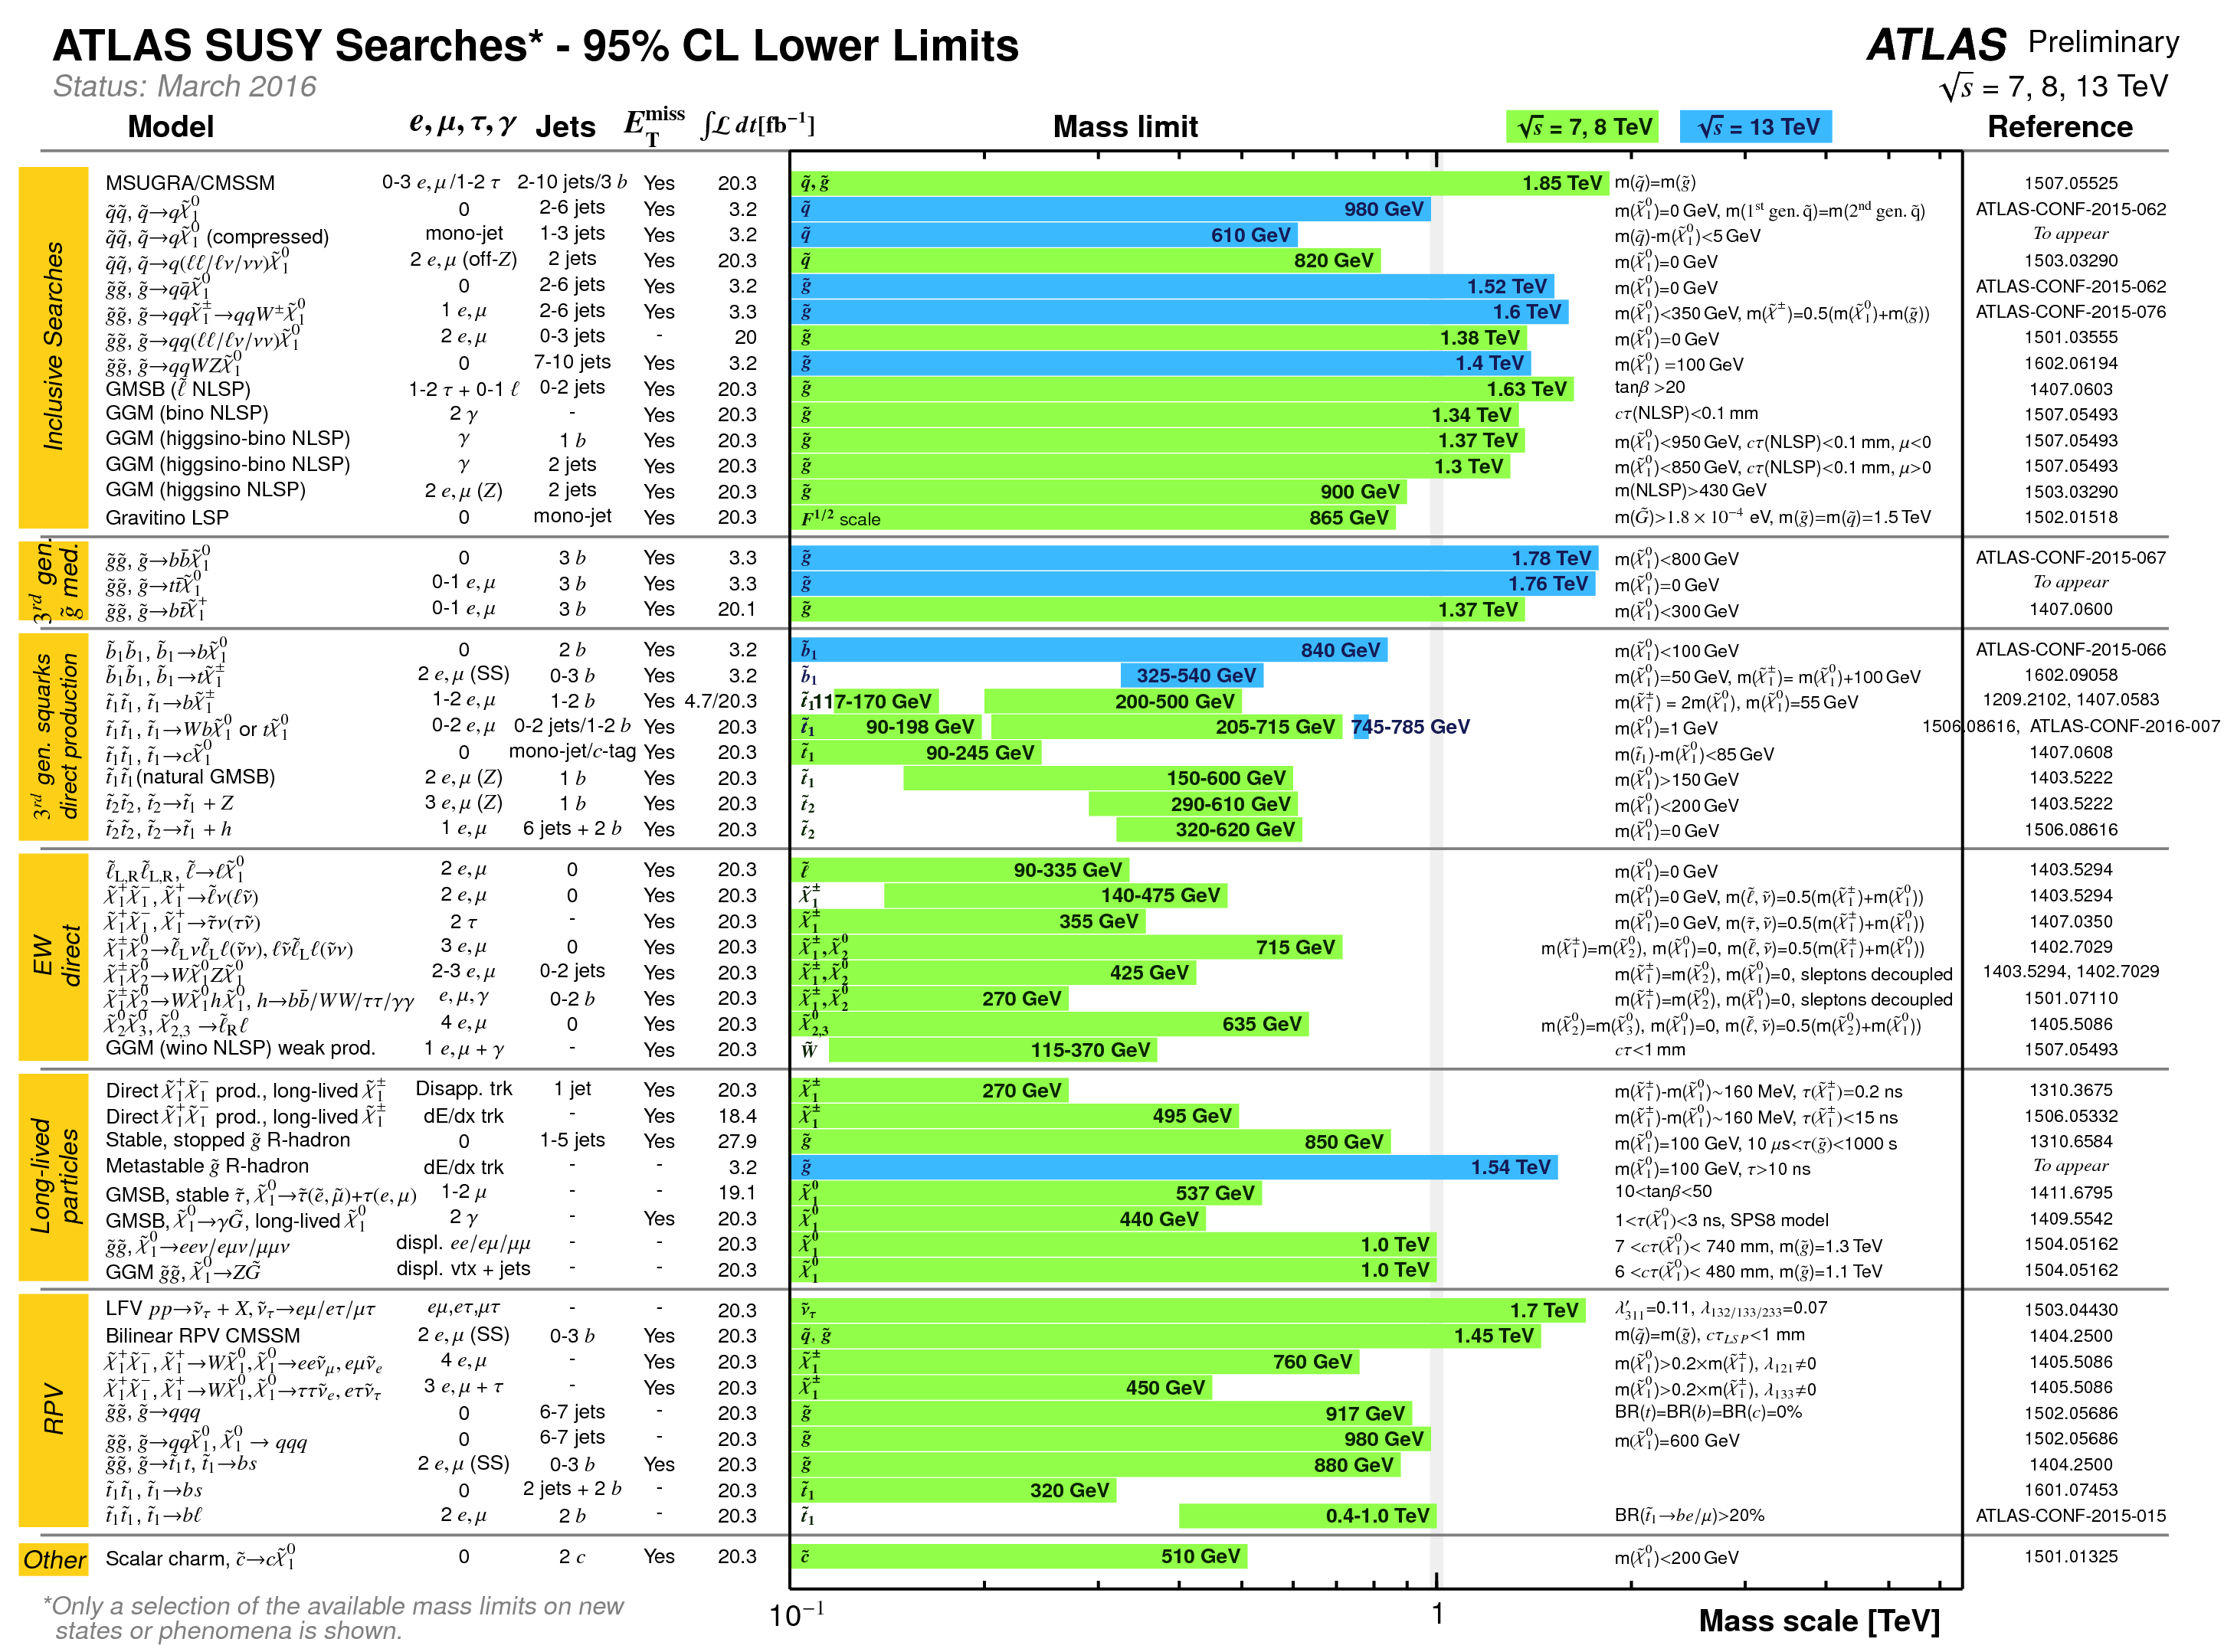
\includegraphics[width=\textwidth]{Chap3/ATLAS_SUSY_Summary.png}
\caption[Exclusion limits of ATLAS searches for Supersymmetry]{Exclusion limits of ATLAS searches for Supersymmetry. Squark and gluon masses are predominantly above the 1 TeV. \citep{SUSYlimits}}
\label{fig:SUSYlimit}
\end{sidewaysfigure}
\cleardoublepage


So far searches in the electroweak region have been unable to find evidence of supersymmetric particles. Limits on their masses according to various decay scenarios have been obtained and can be seen in Fig \ref{fig:summaryplot}.
\begin{figure}[!ht]
	\centering
	\captionsetup{width=0.8\textwidth}
	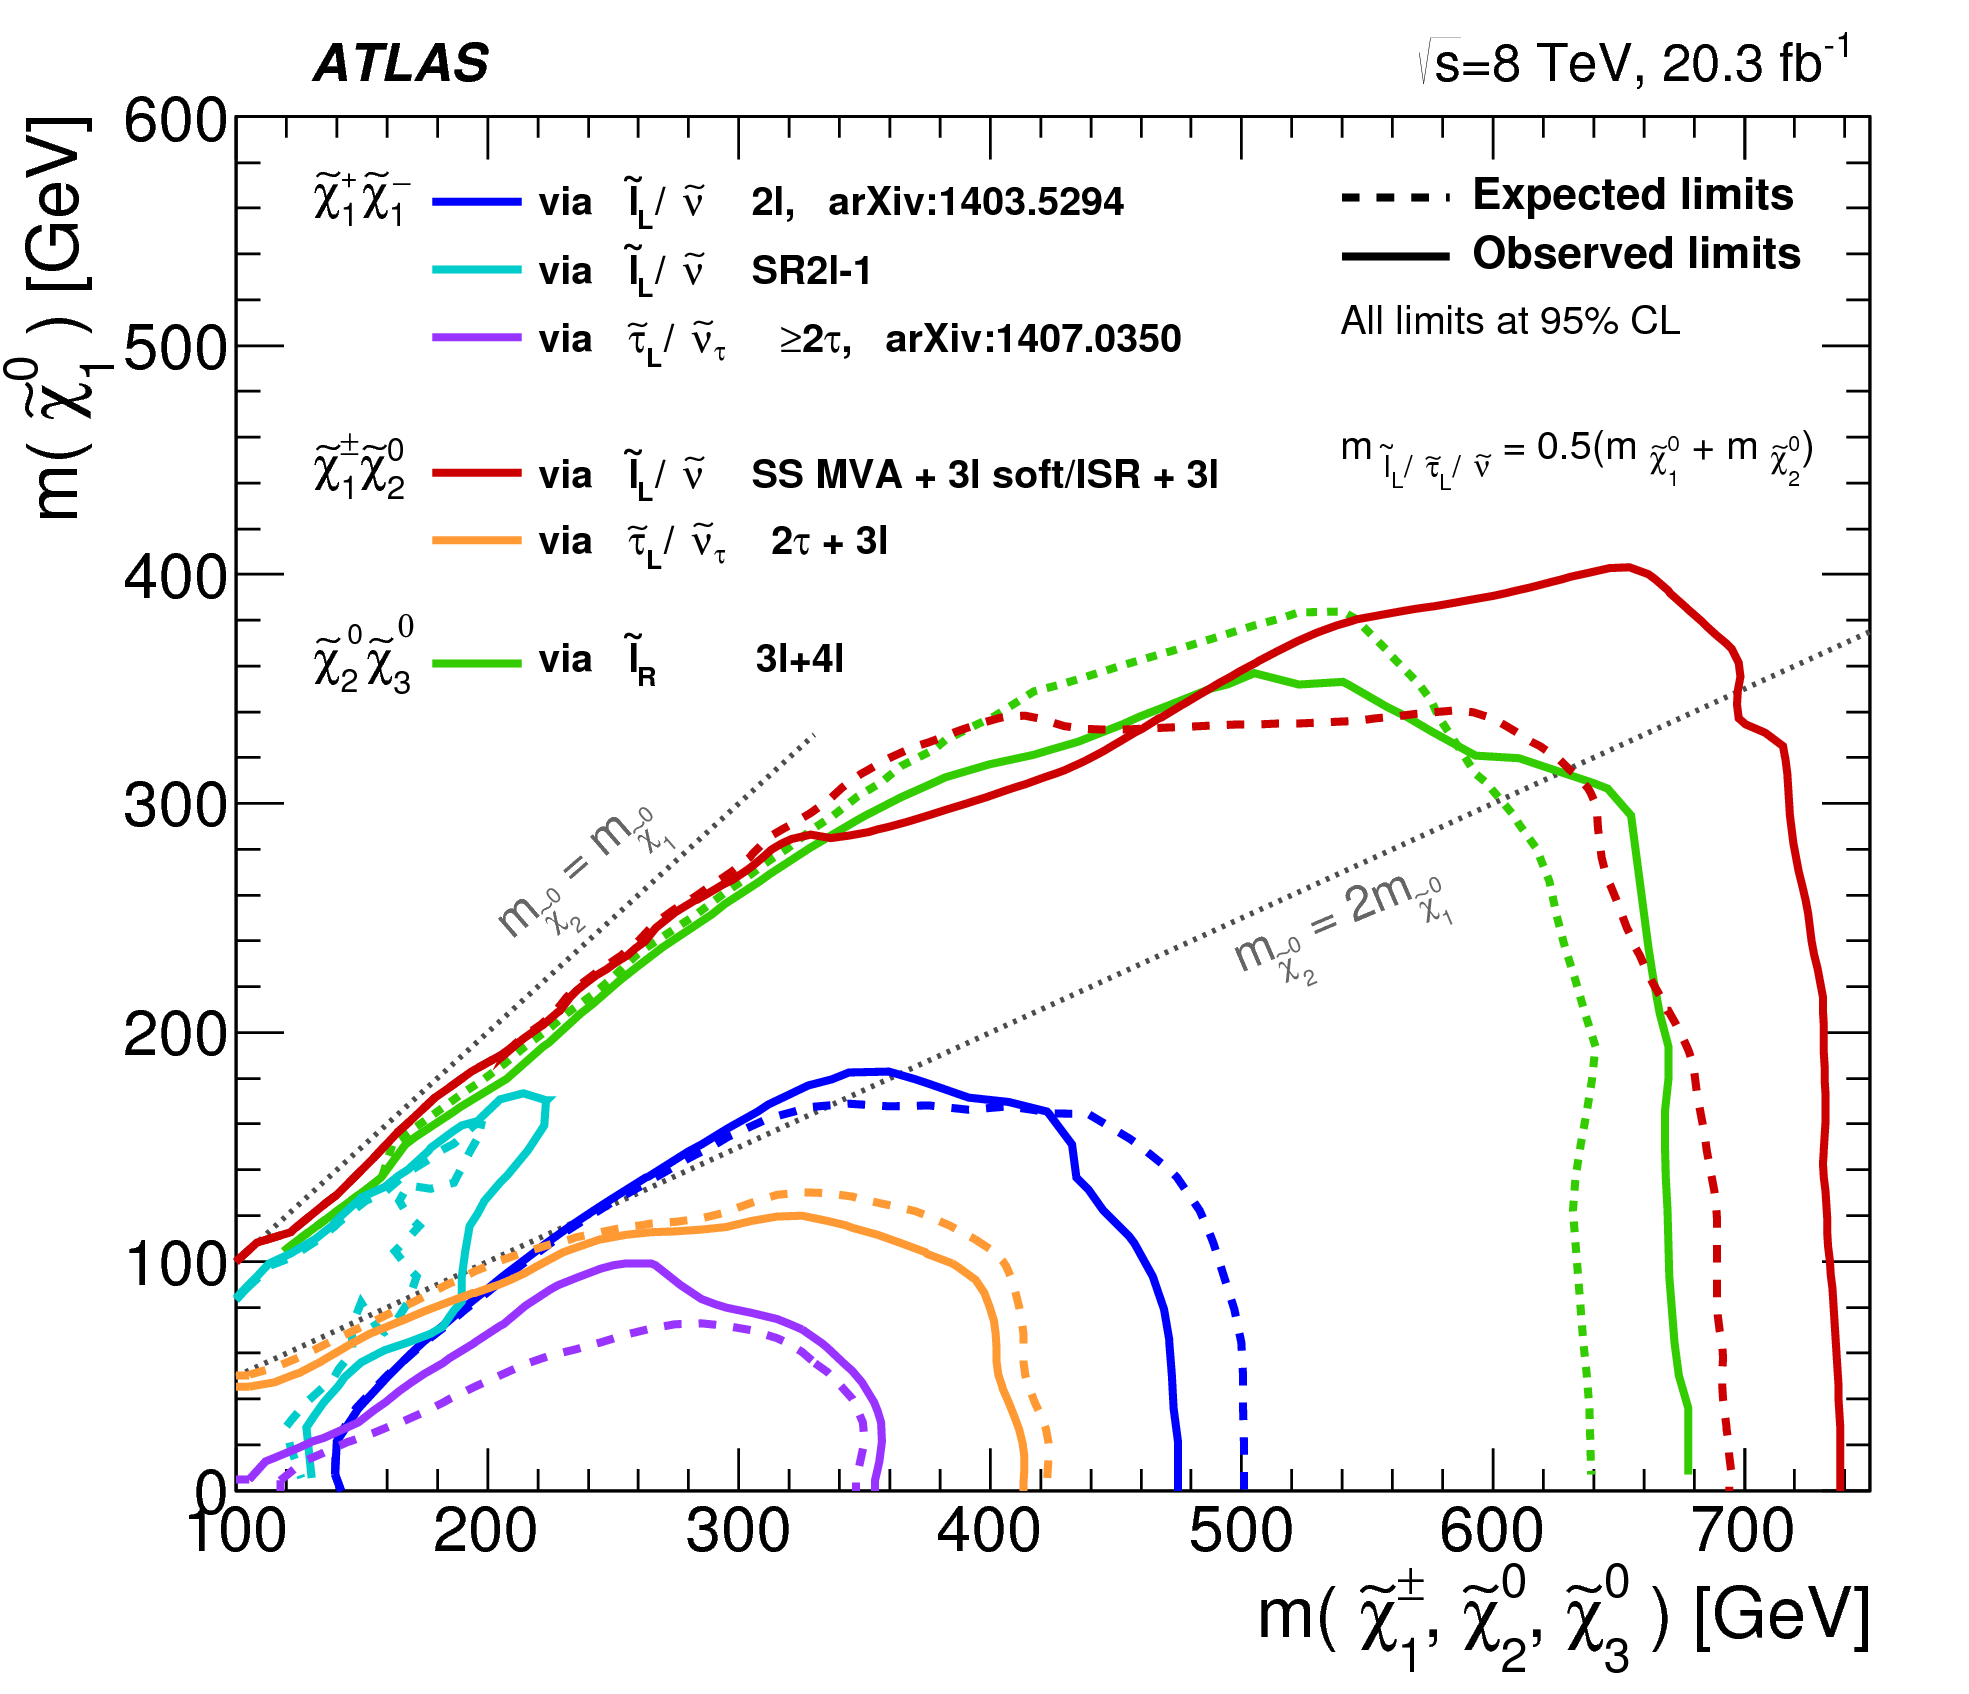
\includegraphics[scale=0.12]{Chap3/fig_19b}
	\caption[Exlcusion limits on electroweak production at ATLAS]{The 95\% CL exclusion limits on $\chi_1^+\chi_1^-$, $\chi_1^{\pm}\chi_2^0$ and $\chi_2^0\chi_3^0$ production with $\tilde{\ell}$-mediated decays, as a function of the $\chi_1^{\pm},\,\chi_2^0$ and $\chi_1^0$ masses \citep{aad2016search}. }\label{fig:summaryplot}
\end{figure}

These results are taken from the  analysis performed at $\sqrt{s}=$8 TeV and integrated luminosity of 20.3 fb\textsuperscript{-1} \citep{atlas2015search}. The search was performed based on various scenarios of the MSSM, involving electroweak production of charginos and neutralinos. The turquoise and blue lines represent decay scenarios that are relevant for this paper as they show information on slepton-mediated decays of a chargino pair. 
In particular, the production of a  $\tilde{\chi}^{+}_{1}\tilde{\chi}^{-}_{1}$ pair decaying through a slepton ($\tilde{\ell}$) with final states containing two opposite sign leptons will be considered (see Fig. \ref{fig:EWchargino}). 
\begin{figure}[!h]
  \centering   	
  	\captionsetup{width=0.8\textwidth}
	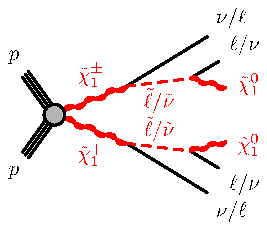
\includegraphics[]{Chap2/C1C1-llvvN1N1-slsnu}	
\caption[Feynman diagram of slepton-mediated chargino decay]{Electroweak chargino pair production in proton-proton collisions with intermediate slepton in the decay process.}\label{fig:EWchargino}
\end{figure}  

In this thesis three different patterns of mass-splitting between the chargino and the neutralino will be considered. Denoted by the pair of numbers assigned to the masses (in GeV) of the chargino and the neutralino respectively, they are 600-100, 400-200, and 200-150 signal models. The choice for these signals is motivated by the fact that they are not covered by the exclusion limits shown in Fig. \ref{fig:EWchargino} and their variety in terms of mass splitting.
For all of them the mass of the intermediate slepton is set to be $m_{\bar{\ell}} = 0.5(m_{\tilde{\chi}_1^{\pm}}+\tilde{\chi}_1^{0})$. 

The cross-section of the investigated production process depends on the mass of the chargino - lighter ones are more likely to be produced and therefore have a larger cross-sections. Fig. \ref{fig:xsec} shows the distribution of the theoretical cross sections depending on the mass of the chargino.
The cross sections for this process were obtained from \citep{Fuks:2012qx,Fuks:2013vua}. 

\begin{figure}[!h]
\centering
 \captionsetup{width=0.8\textwidth}
	\includegraphics[scale=0.4]{Chap3/c1c1_wino}
	\caption{The distribution of cross-sections for slepton-mediated chargino decay \citep{xsec}.}
	\label{fig:xsec}
\end{figure}

In the nomenclature used at LHC and in this thesis, electrons and muons are called ``light leptons". Taus are considered separately as they decay very promptly and therefore are very difficult to reconstruct. This thesis only focuses on final states containing electrons and muons and thus the designation ``lepton" only refers to these particles.  

 

%However, given that so far only 3.2 fb\textsuperscript{-1} of integrated luminosity has been achieved at $\sqrt{s} = 13$ TeV.

\section{General search methods}
Detecting new physics events at LHC requires using computational and statistical methods that can deal with the type of information a particle accelerator produces. The data is initially collected using triggers corresponding to the type of events under analysis. Each event has a large number of physical characteristics such as momentum, energy, mass, multiplicities, etc. The numbers representing them are all stored in a data structure which then can be accessed, modified and analysed using software tools. 

The cornerstone of all accelerator physics analyses is the correct estimation of background events. All background events represent physics that is already known and that has some similar or identical features with the processes under investigation. For instance, this thesis focusses on the reactions that have precisely two oppositely charged leptons in their final states. A number of processes well described by the standard model share this characteristic and therefore will form the background. 

The task of correctly identifying background is therefore crucial in the process of searches for new physics events. Monte Carlo (MC) simulations are used to generate background events distribution samples according to a probability density function of a particular process. In this thesis MC simulated data samples are used to model SM background events along with SUSY signal events. All the samples include events that can result in dileptonic decays. 

The data is then overlaid on the simulated background to see whether there is a disagreement between data and background. If there is a significantly large excess of data over background it can lead to new discoveries such as the existence of a new particle.  The presence of a new particle can reveal itself in a number of ways. The straightforward way to detect a new physics event is an abnormality in some distribution of the data, as was the case with the discovery of the Higgs (see Fig. \ref{Higgs}). The narrow peak over a smooth line in mass distribution of diphoton events constituted a significant excess over the SM predictions and was in agreement with theoretical predictions \citep{Aad:2012tfa}. 

\begin{figure}[!h]
	\centering
	\captionsetup{width=0.8\textwidth}
	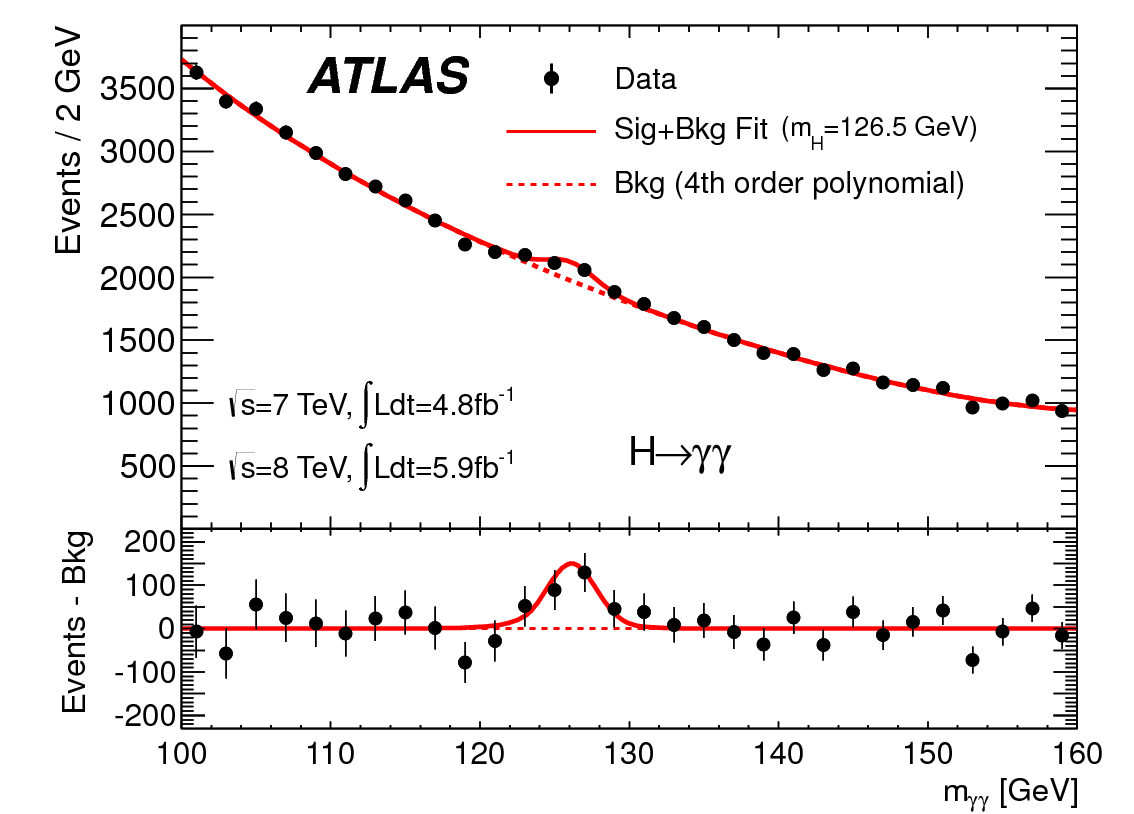
\includegraphics[scale=0.2]{Chap3/figaux_004a}
	\caption[Invariant mass of diphoton events: discovery of the Higgs]{Invariant mass distribution of diphoton 				candidates for the combined $\sqrt{s}$ = 7 TeV and $\sqrt{s}$ = 8 TeV 			data samples. The mass of the Higgs corresponds to the peak at 126.5 				GeV \citep{Aad:2012tfa}.}
	\label{Higgs}
\end{figure}

Unfortunately, this method does not work well for SUSY particles and other techniques have to be used. Standard search techniques involve defining \textbf{signal regions} in data distributions that are sensitive to possible SUSY signals and looking whether there is a significant excess over the SM background predictions in these regions. 
This also includes looking for abnormal tails in distributions of different variables that are not in agreement with the SM predictions. These variables will be discussed in the subsection \ref{subsec:Variables}. Signal regions are usually determined using the ``cut-and-count" approach that will be discussed in the subsection \ref{subsec:stat}.

\section{Overview of background processes}
In order to distinguish new physics events from the SM events it is necessary to be able to suppress all SM events that have the same final state. Within the scope of this thesis that includes events that have precisely two leptons with opposite charge. The processes described in this section constitute MC simulated background that was used in the search for signal regions.

The $Z$+jets background comes from the production of jets of particles in association with a $Z$ boson or a virtual photon (Drell-Yan process), which then decays into two leptons. $t\bar{t}$ pair creation is a common process in $pp$ collisions and is one of the dominant processes in dilepton decays. The quark-antiquark pair decays via the $W^+bW^-\bar{b}$ intermediate state into three different final states with either no leptons, one lepton, or two leptons (here leptons include the tau). The latter decay cascade is $t\bar{t} \to W^+bW^-\bar{b} \to \ell \nu \ell \nu b \bar{b}$. Final states that include electrons and muons constitute around 5\% of the entire $t\bar{t}$ production \citep{Wagner:2010wd}. Thus, the $t\bar{t}$ production is one of the main background processes in searches for BSM events in various channels, not only those involving two-lepton final states. 

The diboson production channel is dominated by the production of the $WW$ pair with subsequent decay into two lepton/neutrino pairs. Contributions also come from the $ZV$ channel, where $V = W$ or $Z$.
Other sources of dilepton final states are $W$+jets and single-top quark production processes. Both of them have a decay channel with final states containing a lepton and a neutrino, however their overall contribution to the background is small compared to diboson, $t\bar{t}$, and $Z$+jets. 
All the MC background predictions used in this thesis belong to one of the categories described in this section. 

A serious hindrance in LHC analyses is the phenomenon of ``pileup".  Among the collisions that produce events of interest there are additional collisions that contaminate the output with extra jets. Along with this, tighter spacing between bunches means that for a specific collision, additional jets might originate from a neighbouring collision as the sensitivity windows for many ATLAS subsystems are longer than 25 ns \citep{Marshall:2014mza}. Dealing with the increased pileup presents an additional challenge at the $\sqrt{s}=13$ TeV run, because of additional jet contamination of the data. 

%Many of the subsystems have sensitivity windows longer than 25 ns, which is the interval between proton-proton bunch crossings.




\section{Event selection and $b$-tagging}

Event reconstruction is the process of turning raw data into manageable format that includes quantities needed in physics analysis. An event has to pass certain identification criteria to be chosen for reconstruction. Correct identification of different physics objects at LHC includes a large number of dedicated algorithms which are not presented in this thesis, but are available elsewhere \citep{Aad:2016tuk}. 
However, in this section a very general outline of the selection procedure for reactions that result in two leptonic decays will be given. All ``signal" objects have to pass a set of criteria to obtain a high quality sample with minimum possible contamination.

Signal electrons are required to have $|\eta|<2.47$ and transverse momentum $p_{T}>10$ GeV. These are inferred from the calibrated  energy deposits in the EmCal and must have a matching ID track. Signal muons are reconstructed using information from MS and ID tracks and are required to have   $|\eta|<2.5$ and $p_{T}>10$ GeV. Jets are reconstructed using information from calorimeters and are divided into ``central" and ``forward" categories. Central jets must have $|\eta|<2.4$ and $p_{T}>20$ GeV. Forward jets are those with $2.4<|\eta|<4.5$ and $p_{T}>30$ GeV. 

One of the common techniques used in LHC analyses is the identification of central jets that have $b$-hadrons (hadrons containing bottom quark/s).  These jets are referred to as $b$-tagged and are identified using multivariate techniques based on machine learning instruments such as artificial neural networks and boosted decision trees \citep{Aad:2015ydr}. The efficiency of $b$-tagging has been significantly improved in run-II due to the addition of the Insertable B-Layer in the ID. $b$-tagging is an extremely useful technique because some important heavy particles such as top quark and the Higgs decay into bottom quarks.  

\subsection{Event variables used in the analysis}
\label{subsec:Variables}

A set of discriminating variables associated with searches for evidence of SUSY is presented here. Topological and kinematic variables as well as quantities derived from them will be investigated.

\begin{itemize}[leftmargin=0cm]
\item[]$\bm{p^X_T}$ The transverse momentum of an object $X$.
\item[]$\bm{\Delta\phi(X,Y)}$ The difference in the azimuthal angle between two reconstructed objects $X$ and $Y$, e.g. ${\Delta\phi(E_{\text T}^{miss},\ell)}$.
\item[]$\bm{E_{\text T}^{\text {miss}}}$ The magnitude of the missing transverse momentum of the event. Missing transverse momentum is defined as the negative vector sum of the transverse momenta of all identified objects.
\item[]$\bm{E^{\text{miss,rel}}_{\text T}}$ This value is defined as 
\[
 E_{\text T}^{\text {miss,rel}} = 
  \begin{cases} 
   E_{\text T}^{\text {miss}}\quad & \text{if } \Delta\phi(E_{\text T}^{\text {miss}},\ell/j) \geq \pi/2, \\
   E_{\text T}^{\text {miss}}\times \text{sin}\Delta\phi(E_{\text T}^{\text {miss}},\ell/j) \quad      & \text{if } \Delta\phi(E_{\text T}^{\text {miss}},\ell/j)<\pi/2
  \end{cases}
\]
where $\Delta\phi(E_{\text T}^{\text {miss}},\ell/j)$ is the azimuthal angle between the direction of $E_{\text T}^{\text {miss,rel}}$ and that of the nearest electron, muon, or central jet. 
\item[]$\bm{m_{\ell \ell}}$ The invariant mass of the two leptons.
\end{itemize}

Another derived event variable is the so-called ``stransverse mass"  $m_{\text {T2}}$ which was introduced as a way to infer information about undetected particles \citep{Lester:1999tx,Barr:2003rg}. Along with that, it is also proved useful in suppressing backgrounds. It is used to bound the masses of a pair of supersymmetric particles each of them decaying into one visible and one invisible particle. It is a function of the momenta of two visible particles and the missing transverse momentum of an event. Its abbreviated mathematical description is as follows
\begin{equation}
m_{\text{T2}} = \min_{\mathbf{q}_{\text T}}\Big [\max \Big ( m_{\text T} (\mathbf{p}_{\text T}^{\ell 1},\mathbf{q}_{\text T}),m_{\text T}(\mathbf{p}_{\text T}^{\ell 2},\mathbf{p}_{\text T}^{\text{miss}}-\mathbf{q}_{\text T}) \Big ) \Big ] ,
\end{equation}
where $\mathbf{p}_{\text T}^{\ell 1}$ and $\mathbf{p}_{\text T}^{\ell 2}$ are the transverse momenta of the two leptons, and $ \mathbf{q}_{\text T}$ is a transverse vector that minimizes the larger of two transverse masses $m_{\text T}$ which is defined as
\begin{equation}
m_{\text T}(\mathbf{p}_{\text T},\mathbf{q}_{\text T}) = \sqrt{2(p_{\text T}q_{\text T} - \mathbf{p}_{\text T} \cdot \mathbf{q}_{\text T})}.
\end{equation}

The $m_{\text{T2}}$ has an upper end at the $W$ mass for SM $t\bar{t}$ and $WW$ events, where the missing momentum originates from neutrinos. In case with signal events, where the LSP contributes to $ \mathbf{p}_{\text T}^{\text{miss}}$, the $m_{\text{T2}}$ endpoint is correlated to the mass difference between the chargino and the lightest neutralino. $m_{\text{T2}}$ is more sensitive to large mass splittings as its distribution then extends significantly beyond the distributions of $t\bar{t}$ and $WW$ events. Its performance decreases for signals with small mass splittings.  

\section{Cut-and-count approach and test statistics}
\label{subsec:stat}
As discussed previously, a good signal region retains as many signal events as possible while at the same time cutting off background events. The way to suppress the background is to use successive cuts. The cuts are based on determining physical quantities that are able to discriminate between signal and background. The choice for a single cut is motivated both by theoretical considerations and the shapes of the MC signal and background distributions. 

To optimize a cut or a set of cuts a metric that shows their discriminating power is needed. The numerical expression of how well a cut performs is given by a score function and its result will be referred to as ``significance". The score function is constructed in the following way.
The total number of events in a particular selection is $N$, and it is the sum of $S$ and $B$. The latter two refer to the number of signal and background events respectively. This gives the following expression
\begin{equation}
S = N -B
\end{equation}
The uncertainty of $S$ is then
\begin{equation}
\sigma^2(S) = \sigma^2(N) + \sigma^2(B) = N+\sigma^2(B).
\end{equation}
$N$ is a mean value of a distribution described by Poisson statistics where the uncertainty is $\sigma = \sqrt{\lambda}$, so squaring it back just yields $N$. 
$\sigma(B)$ is the uncertainty on the estimated average of the $B$ value. 
Because estimation of the background is done with large MC statistics the $\sigma(B)$ in this case can be treated as negligible. So what is left is
\begin{equation}
\frac{S}{\sigma(S)} = \frac{S}{\sqrt{N}} = \frac{S}{\sqrt{S+B}}.
\end{equation}
This determines the number of standard deviations away from the 0 of the signal. Due to SUSY signals being very small compared to the background, further simplification can be done, so that the above expression becomes
\begin{equation}
\frac{S}{\sigma(S)}\simeq \frac{S}{\sqrt{B}}.
\end{equation} 

The process of scientific discovery relies predominantly on using statistical methods to justify new discoveries and safeguard against false ones. It is especially important in HEP as it operates on quantum level where almost everything is described using probabilistic arguments (a particle's wave function being the most obvious example).
  
Any potential discovery in HEP must comply with stringent requirements posed by statistical inference. If some signal has a mean that is away from the mean of the background-only sample by three standard deviations (3$\sigma$), it is referred to as ``evidence". If it is a 5$\sigma$ event then it is claimed as a discovery. To put this into perspective, the chance of a 5$\sigma$ event being just random fluctuation is around 1 in 3.5 million. 
The expression $S/\sqrt{B}$ thus is a rough estimate of the number of standard deviations and can serve as a metric to assess the quality of candidate signal regions. 

A very important point about the $S/\sqrt{B}$ is that it grows with the increase in luminosity $\mathcal{L}$ at the rate of $\sqrt{\mathcal{L}}$. This can be used in extrapolating its values for higher projected luminosities that are going to be achieved in the 13 TeV run-II at the LHC.

\section{Computational tools}
Most of the HEP analyses are performed with ROOT framework which was developed at CERN specifically for this purpose \citep{root}. It is a multi-purpose package that provides tools for big data processing, statistical analysis, visualisation and storage. It is written in C++ programming language, but also provides integration with other languages such as Python, Ruby, R, etc.  ROOT is especially convenient because it provides constructors and methods created specifically for the LHC geometry and the type of analyses it entails. All the computational manipulations and visualisations were performed in ROOT using applications written in C++ and Python. 




 

